\documentclass[tikz,border=10pt]{standalone}
\usetikzlibrary{calc}
% Scale s = 0.022346 cm/px; origin at A, y measured upward
\begin{document}
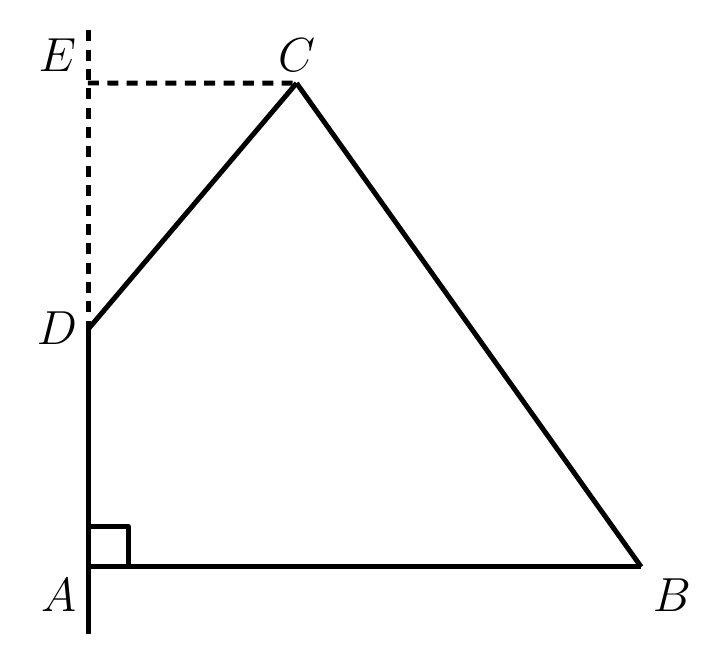
\begin{tikzpicture}[line join=round, line width=1.8pt,
  % auxiliary dashed style: dash pattern on 4pt off 3pt
  auxdash/.style={dash pattern=on 4pt off 3pt}]
  % Named coordinates (converted from pixels)
  \coordinate (A) at (0,0);
  \coordinate (B) at (7.026,0);
  \coordinate (C) at (2.650,6.143);
  \coordinate (D) at (0.011,3.028);
  \coordinate (E) at (0,6.145);
  \coordinate (Dstub) at (0.011,-0.849);   % DA stub below A
  \coordinate (Etop) at (0.011,6.816);     % dashed stub above E, top at y=36 px

  % Solid segments
  \draw (A) -- (B);
  \draw (B) -- (C);
  \draw (C) -- (D);
  \draw (D) -- (Dstub);

  % Dashed auxiliary segments (EC, ED and stub above E)
  \draw[auxdash] (E) -- (C);
  \draw[auxdash] (Etop) -- (D);

  % Right-angle mark at A (side about 23 px = 0.514 cm)
  \draw (0.514,0) -- (0.514,0.514) -- (0,0.514);

  % Labels (plain math, no \boldmath)
  \node[font=\fontsize{17.5}{21}\selectfont, below left] at (A) {$A$};
  \node[font=\fontsize{17.5}{21}\selectfont, below right] at (B) {$B$};
  \node[font=\fontsize{17.5}{21}\selectfont, above] at (C) {$C$};
  \node[font=\fontsize{17.5}{21}\selectfont, left] at (D) {$D$};
  \node[font=\fontsize{17.5}{21}\selectfont, above left] at (E) {$E$};
\end{tikzpicture}
\end{document}